%%%%%%%%%%%%%%%%%%%%%%%%%%%%%%%%%%%%%%%%%%%%%%%%%%%%%%%%%%%%%%%%%%%%%%%%%%%%%%%%%%%%%%%%%%%%%%%%%%%
%%%%%%%%%%%%%%%%%%%%%%%%%%%%%%%%%%%%%%%%%%%%%%%%%%%%%%%%%%%%%%%%%%%%%%%%%%%%%%%%%%%%%%%%%%%%%%%%%%%

\chapter{Introducción}

Gracias a los avances médicos del último siglo se ha incrementado la esperanza de vida y la 
calidad de vida. Desafortunadamente, también ha aumentado la presencia de enfermedades 
no-transmisibles asociadas con la edad. 
%
Para muchas de esas enfermedades no se han identificado factores causales o curas definitivas 
\cite{PlanAlzheimer04}.
%
En México el sector de la población con más de 60 años de edad (aquellos con alto riesgo para este
tipo de enfermedades) contempló a 10 millones de personas en 2010 y en 2015 esta cifra 
creció a 12 millones \cite{Censo10,Intercensal15}.

De entre las enfermedades ante las cuales este grupo de edad es vulnerable, en este trabajo se 
destaca la demencia. 
%
La demencia consiste en el desarrollo de déficit cognoscitivos suficientemente graves como para 
interferir en las actividades laborales y sociales.
%
El deterioro cognitivo característico de la demencia se considera irreversible, debido a lo cual 
ha surgido un gran interés en definir y diagnosticar etapas tempranas de este padecimiento con el 
fin de evitar en lo posible dicho síntoma \cite{Knopman01}.

Se define entonces al deterioro cognitivo leve (DCL) como ``\textit{ una alteración adquirida y 
prolongada de una o varias funciones cognitivas, que no corresponde a un síndrome focal y no cumple 
criterios suficientes de gravedad para ser calificada como demencia "} \cite{Robles02}.
%
No hay un consenso absoluto sobre qué deficiencias cognitivas --o más bien en qué grado-- 
distinguen a un individuo con DCL, de modo que hay una multitud de definiciones que no son
equivalentes \cite{Petersen01}.
%
En el presente trabajo se desarrollaron métodos para caracterizar con DCL adultos mayores comparados 
con sanos en base a mediciones objetivas, pero manteniendo presente que el fenómeno del deterioro 
cognitivo no puede reducirse exclusivamente a tales mediciones. Las conclusiones sobre las señales
electrofisiológicas deben ser contrastadas, por ejemplo, con los resultados de evaluaciones 
neuropsicológicas y revisiones neurológicas.

En concreto se utilizarán registros de varias señales electrofisiológicas --incluyendo 
electroencefalograma (EEG), electrooculograma (EOG) y electromiograma (EMG)-- obtenidos durante 
etapas específicas en el sueño del paciente, técnica conocida como polisomnografía (PSG)\footnote{La 
PSG puede contener otro tipo de registros como electrocardiograma, niveles de oxígeno en la sangre, 
esfuerzo respiratorio, entre otros}.
%
Conviene destacar que muchos de los marcadores para el DCL definidos en base al EEG, dependen
efectivamente de su respectivo espectro de potencias; el razonamiento usual para ello es que si el 
EEG está asociado al grado de actividad cerebral en términos de energía, entonces el espectro de 
potencias explica \textit{cómo} es dicha actividad.

El presente trabajo toma parte en el problema metodológico de que las señales 
electrofisiológicas típicamente representan procesos no--lineales y \textbf{no--estacionarios}, y sin 
embargo suelen ser analizadas usando herramientas que suponen linealidad y estacionariedad. Se sabe que
las señales biológicas son globalmente no estacionarias, pero en ventanas pequeñas de tiempo estas son
mayormente estacionarias. Además estudios previos han demostrado que análisis de señales en tiempos
intermedios pueden ayudar a inferir problemas neurológicos \cite{Cohen77}.
%
En el caso particular del espectro de potencias, es común que sea calculado usando la 
transformada de Fourier sobre segmentos cortos para evitar los \textit{efectos} de la 
no--estacionariedad \cite{Kaiser00}.
%
A consecuencia de lo anterior los datos pueden contener información \textit{oculta}, o incluso 
pueden llegar a no ser representativos del fenómeno que se estudia. 
%
Es por ello que se buscan herramientas para verificar la estacionariedad débil (más detalles en 
la sección de métodos)  en los registros electrofisiológicas, y con especial atención en la 
posibilidad de que puedan usarse como marcadores de deterioro cognitivo.
%
Adicionalmente, la posibilidad de que sujetos con PDC exhiben estacionariedad débil en sus 
registros de EEG en mayor proporción (respecto a individuos sanos) fue sugerida anteriormente
\cite{Cohen77}. En esta tesis probable DCL o PDC, se asume que solo las pruebas neurológicas
son lo determinan.

%%%%%%%%%%%%%%%%%%%%%%%%%%%%%%%%%%%%%%%%%%%%%%%%%%%%%%%%%%%%%%%%%%%%%%%%%%%%%%%%%%%%%%%%%%%%%%%%%%%
%%%%%%%%%%%%%%%%%%%%%%%%%%%%%%%%%%%%%%%%%%%%%%%%%%%%%%%%%%%%%%%%%%%%%%%%%%%%%%%%%%%%%%%%%%%%%%%%%%%

\section{Antecedentes}

La epoca del sueño de Movimientos Oculares Rápidos (MOR) ha demostrado ser un indicador del DC en los adultos mayores. En otros estudios, se ha encontrado una mayor potencia absoluta y relativa en frecuencias lentas, en regiones laterales \cite{Brayet} y menos atonía muscular \cite{Chen}.

Los estudios anteriores han incluido análisis lineales del Electroencefalograma (EEG) o del Electromiograma (EMG), pero el Electrooculograma (EOG) no se ha considerado como un posible marcador de deterioro cognitivo. Los tres indicadores de sueño MOR aparecen generalmente en orden consecutivo. Al ingresar a esta etapa, los husos y las ondas lentas de alta amplitud están ausentes, el EEG tiene abundantes frecuencias beta y gamma \cite{SteriadeIntracortical1996,Llinas}, hay una abrupta pérdida de voltaje que ocurre en un intervalo menos de 2 segundos \cite{Rosales-Lagarde2009}, y, luego, aparcen los movimientos oculares (MOR) característicos \cite{AASM07,Rechtshaffen1968}.
%\cite{Aserinsky,AASM07,Rechtshaffen1968}.

El sueño MOR se ha asociado durante mucho tiempo con las funciones cognitivas \cite{Moruzzi1963}; 
citado en \cite{Corsi1983}. El sueño MOR desempeña un papel en la consolidación de la memoria 
\cite{Lucero, Leconte1971, Leconte1972, Fishbein1971, Fishbein1977, Pearlman1971, Pearlman1973, Pearlman1974, Smith}.
Después de tareas complejas, hay reactivaciones de circuitos neuronales durante MOR sleep \cite{Louie}. 
La Potenciación a Largo Plazo (LTP) solo ocurre durante la vigilia y el sueño MOR, y, dependiendo de su fase theta del hipocampo, la LTP puede mejorarse o inhibirse \cite{Pavlides1988}.


El sueño MOR mejora la memoria y los procesos de atención mediante las entradas colinérgicas \cite{Braun} a través de pontine \cite{Datta2004} y las estructuras del basales del cerebro anterior \cite{Blake}. Durante el envejecimiento normal y especialmente durante el envejecimiento patológico, los procesos de atención y memoria se vuelven más vulnerables, y las neuronas colinérgicas son las más afectadas \cite{Schliebs2011}. El envejecimiento afecta a varias estructuras anatómicas que resultan en la pérdida de un eje dendrítico en las neuronas corticales que muestran una degradación en su complejidad fractal estructural \cite{Lipsitz}.

En otros países, el deterioro cognitivo leve (DCL) ha sido medido por el Instituto Nacional de Enfermedades
Neurológicas y Comunicativas y la Asociación de Stroke / Alzheimer's Disease and Related Disorders o NINCDS ADRDA criteria \cite{McKhann}. Sin embargo, las pruebas neuropsicológicas empleadas en estos estudios todavía no se han validado en México debido en parte a la alta tasa de analfabetismo entre los adultos mayores, que en México asciende
al 25.6 \% \cite{CONAPO2010}. En cambio, en estudios epidemiológicos, el Examen Cognitivo Transcultural (CCCE) y otras pruebas se han utilizado \cite{Rosales-Lagarde2016}. El CCCE muestra una prevalencia del 28.7 \% de deterioro cognitivo sin demencia (DCSD) que aumenta con la edad y disminuye con un nivel educativo más alto \cite{Mejia-Arango2011}. La prueba de Neuropsi, desarrollada en la UNAM, también ha distinguido claramente entre sujetos normales, con deterioro cognitivo y demenciales \cite{Ostrosky1999, Abrisqueta, Montes2012}. En el presente estudio, una puntuación de 3 desviaciones estándar por debajo de la media en la prueba de Neuropsi se consideró una indicación de Probable DC (PDC).

En un estudio reciente, EEG de una noche polisomnografía de personas mayores con y sin deterioro cognitivo según las evaluaciones con el Neuropsi analizó el porcentaje de estacionariedad.  En sueño MOR el porcentaje fue menor que el del sueño NMOR y la vigilia, se obtuvo estacionariedad  como un índice para comparar NMOR versus sueño MOR en ambos grupos \cite{ROSALESLAGARDE2017}.

\section{Antecedentes previo}

El sueño MOR ha sido ampliamente reconocido como parte de la consolidación de la memoria, así como
otras funciones cognitivas 
\cite{Fishbein1971,Fishbein1977,Lucero1970,Pearlman1971,Pearlman1974,Smith1991}.
%
En el caso de adultos mayores, la correlación entre deterioro cognitivo y trastornos del sueño ha 
sido reportada por varios autores a partir de estudios poblacionales 
\cite{Amer13,Miyata13,Reid06,Potvin12}.
%
Tal correlación era de esperarse ya que los procesos de atención y memoria, por ejemplo, dependen de 
los circuitos colinérgicos activados durante el sueño MOR \cite{Braun1997}; estos circuitos son 
propensos a degradación estructural tanto en el envejecimiento normal como en el patológico,  y 
especialmente en el segundo \cite{Schliebs11}.

En 2016 Vázquez-Tagle y colaboradores estudiaron la epidemiología del DCL en adultos mayores dentro 
del estado de Hidalgo y su posible relación con trastornos de sueño, encontrando efectivamente una 
correlación entre una menor eficiencia del sueño (porcentaje de tiempo de sueño respecto al tiempo 
en cama) y la presencia de deterioro cognitivo \cite{VazquezTagle16}.
%
En aquél estudio se efectuaron registros de PSG para algunos de los participantes, con la intención 
de verificar que existen diferencias en los registros correspondientes a individuos con y sin DCL.
%
El presente trabajo se enmarca dentro de una reciente colaboración, con el objetivo de identificar concretamente
los posibles cambios en los registros de PSG  ocurridos durante el DCL o PDC.

La idea de que sujetos con deterioro cognitivo exhiban cambios en sus registros de PSG relacionados 
a la estacionariedad débil, fue sugerida por Cohen en 1977 \cite{Cohen77}; aquél análisis se 
refiere a su vez a trabajos anteriores sobre estacionariedad y normalidad en registros de EEG
\cite{McEwen75,Sugimoto78,Kawabata73}.
%
Los estudios referidos se enmarcan en un primer intento de verificar que los registros 
electrofisiológicos no pueden modelarse como señales \textit{simples} (lo contrario a señales 
complejas).
%
%El tema de la estacionariedad en señales parece relevante nuevamente a la luz de una revisión
%por Kreuz y colaboradores \cite{Kreuz07}, según la cual el método más eficaz para detectar 
%correlación es la correlación \textit{clásica} --en comparación con algunos métodos basados en 
%entropía o información mutua, por ejemplo. 
%%
%Para llegar a tal conclusión analizaron algunos tipos \textit{comunes} de datos, experimentales y 
%simulados, así como algunos tipos comunes de perturbaciones.
%
%Un resultado tan controversial provoca replantearse, por ejemplo, si algún método en particular es 
%adecuado para un tipo arbitrario de datos, o si algunas generalizaciones para estos métodos son 
%efectivamente necesarias.

%%%%%%%%%%%%%%%%%%%%%%%%%%%%%%%%%%%%%%%%%%%%%%%%%%%%%%%%%%%%%%%%%%%%%%%%%%%%%%%%%%%%%%%%%%%%%%%%%%%
%%%%%%%%%%%%%%%%%%%%%%%%%%%%%%%%%%%%%%%%%%%%%%%%%%%%%%%%%%%%%%%%%%%%%%%%%%%%%%%%%%%%%%%%%%%%%%%%%%%

\section{Pregunta de investigación}

¿Los registros de polisomnograma en adultos mayores pueden considerarse como series de tiempo 
débilmente estacionarias? 


%
¿Es posible que la estacionariedad se vea influida por el estado cognitivo del sujeto?

%%%%%%%%%%%%%%%%%%%%%%%%%%%%%%%%%%%%%%%%%%%%%%%%%%%%%%%%%%%%%%%%%%%%%%%%%%%%%%%%%%%%%%%%%%%%%%%%%%%
%%%%%%%%%%%%%%%%%%%%%%%%%%%%%%%%%%%%%%%%%%%%%%%%%%%%%%%%%%%%%%%%%%%%%%%%%%%%%%%%%%%%%%%%%%%%%%%%%%%

\subsection{Hipótesis}

Existen diferencias en la actividad eléctrica cerebral en adultos mayores con DCL, respecto a 
individuos sanos, y es posible detectar dichas diferencias como una mayor o menor 
\textit{presencia} de estacionariedad débil en registros de PSG durante el sueño profundo.

%%%%%%%%%%%%%%%%%%%%%%%%%%%%%%%%%%%%%%%%%%%%%%%%%%%%%%%%%%%%%%%%%%%%%%%%%%%%%%%%%%%%%%%%%%%%%%%%%%%

\subsection{Objetivo general}

Buscar pruebas estadísticas formales para detectar si una serie de tiempo dada procede de un 
proceso estocástico débilmente estacionario.
%
Usar tales pruebas sobre registros de polisomnograma en adultos mayores, para investigar si la 
presencia de segmentos débilmente estacionarios se correlaciona con la condición de probable
deterioro cognitivo.

%%%%%%%%%%%%%%%%%%%%%%%%%%%%%%%%%%%%%%%%%%%%%%%%%%%%%%%%%%%%%%%%%%%%%%%%%%%%%%%%%%%%%%%%%%%%%%%%%%%

\subsection{Objetivos específicos}

\begin{itemize}
\item Estudiar la definición de estacionariedad para procesos estocásticos.

\item Investigar cómo detectar, como prueba de hipótesis, si una serie de tiempo dada proviene
de un proceso estocástico débilmente estacionario, y bajo qué supuestos 
es válida dicha caracterización.

\item Decidir si los registros de PSG, durante sueño profundo, son débilmente estacionarios.

\item Investigar si la presencia de segmentos estacionarios en los registros es diferente si el
PSG corresponde a un individuo con PDCL o PDC.
\end{itemize}


\section{Estructura del texto}

Debido a la naturaleza multidisciplinaria del presente trabajo, se ha estructurado de manera que %resalten los temas teóricos más como objetos abstractos que como componentes de herramientas para el análisis de datos.

El objeto principal de este trabajo es el estudio de la estacionariedad débil en registros de polisomnograma de adultos mayores para investigar si es posible usarlos para

En el primer capítulo se expone una serie de temas concernientes a lo que se ha denominado \textit{estadística en el dominio espectral}, es decir, obtener el espectro de potencias de un proceso estocástico --particularmente de procesos no-estacionarios.
%
Naturalmente, esta tarea implica la exposición de varios otros temas relativos a las condiciones bajo las cuales el espectro de potencias está bien definido, así como las condiciones bajo las cuales es posible su estimación.
%
Debido a la notoria dependencia mutua entre estos temas, se decidió ilustrar en la figura \ref{intro:estructura} la red de temas según dependen unos de otros.

El objetivo final del capítulo es presentar una prueba de estacionariedad débil y que es usada para estudiar las propiedades de los registros.

En el capítulo 2 se describe lo  que es el deterioro cognitivo leve y cómo se detecta a nivel de comportamiento, así como se describen varios esfuerzos por detectar este padecimiento en base a mediciones más objetivas a nivel de sistema (en particular, con el enfoque de mediciones de la actividad cerebral). 
%
Dado que se ha reportado relaciones entre el sueño MOR y la memoria a corto y largo plazo, se dedica una sección a describir el sueño y sus características, y su estudio a través de la polisomnografía.

En el capítulo 3 se muestran los sujetos de estudio; debido a que el trabajo se enmarca en una colaboración, se describe la metodología usada en trabajos anteriores usando esta misma base datos, y se considera como conocidos los datos sobre pruebas neuropsicológicas y los registros de PSG se consideran conocidos. 
%
Posteriormente se expone la metodología original en este trabajo correspondiente en cuanto el uso que se da a la prueba de PSR. El análisis se efectúa en dos niveles: 
\begin{itemize}
\item Para cada sujeto, los registros son segmentados en una colección de ventanas (épocas) que se clasifican como etapas según sus características tipificadas\footnote{Estas características son en su mayoría visuales, y se encuentran reguladas por lineamientos internacionales como aquél de la AASM \cite{AASM07}} , debido a la heterogeneidad del sueño, tiene sentido tratar a estas épocas como una población
\item A nivel de grupo, algunas características son comparadas entre sujetos
\end{itemize}
conviene destacar que la heterogeneidad en los registros puede observarse intuitivamente de manera gráfica.

\begin{figure}
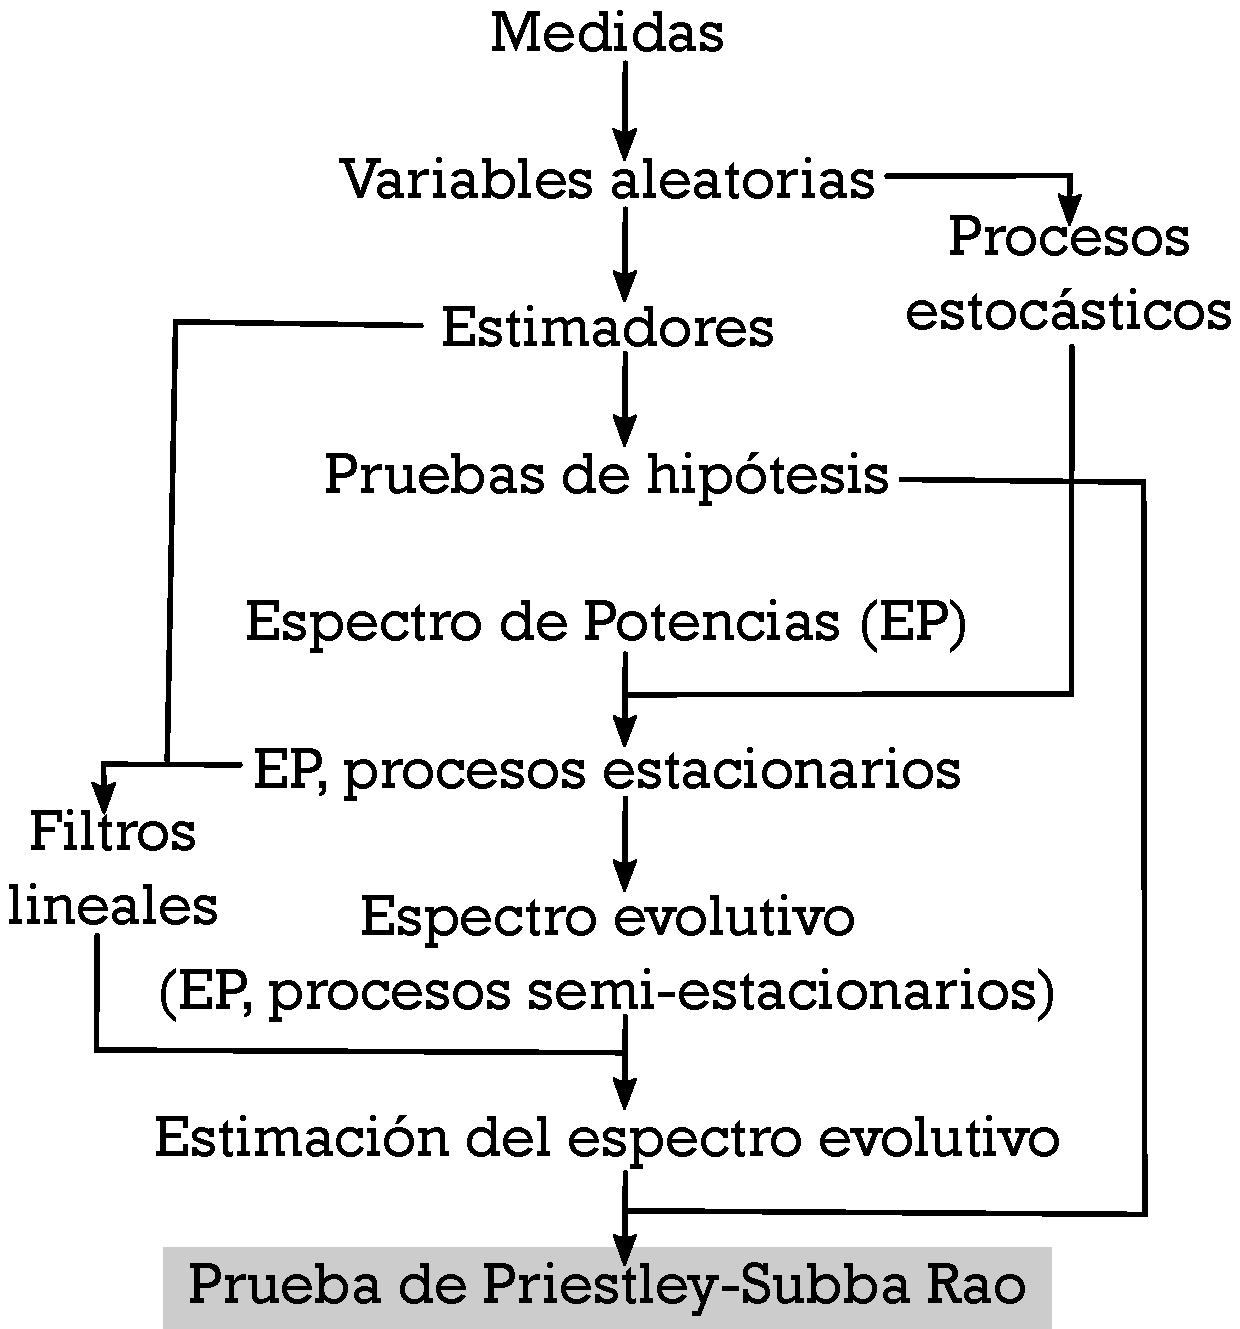
\includegraphics[width=\textwidth]{./estructura_texto.pdf}
\caption{Dependencia de los temas expuestos en el capítulo 1.}
\label{intro:estructura}
\end{figure}

%%%%%%%%%%%%%%%%%%%%%%%%%%%%%%%%%%%%%%%%%%%%%%%%%%%%%%%%%%%%%%%%%%%%%%%%%%%%%%%%%%%%%%%%%%%%%%%%%%%
%%%%%%%%%%%%%%%%%%%%%%%%%%%%%%%%%%%%%%%%%%%%%%%%%%%%%%%%%%%%%%%%%%%%%%%%%%%%%%%%%%%%%%%%%%%%%%%%%%%